\section{Discussion }\label{sec:disc}

The \textbf{principal objective} for natural resource management in Midwest Region NPS units is to emphasize the \emph{grazing ecosystem}, "which is distinguished from other habitats by its prominent herbivore-based food web and by the extent to which ecological processes are regulated by dynamics within that food web. \citep{frank1998}" 
Management objectives that focus on the food web and dynamic trophic interactions between grazers and vegetation as a community contrast with current perspectives, which we found to be overly species-specific (e.g.,the population biology of charismatic and endangered species), and often reactive (e.g., invasive plant species management). 

To be clear, we understand the historical and institutional reasons for these perspectives, and appreciate that continued compliance with federal policy will require much of the species-specific monitoring and reporting to continue. 
But this does not preclude individual NPS units from developing strategies aimed at enhancing the resilience of the grazing ecosystem. 

The \textbf{main strategy} by which we suggest management might better reflect focus on the grazing ecosystem is the \emph{coupling of fire and grazing disturbance regimes} within each unit. 
Our research indicates that compartmentalized management within the region\textemdash e.g., species-specific emphasis on bison population biology and endangered and invasive species, lack of co\"{o}rdination between fire management and vegetation management and monitoring\textemdash currently results in discrete management of fire and grazing, which impedes a multi-trophic grazing ecosystem management strategy. 
Considerable scholarship in rangeland ecology and management describes how the pre-settlement condition of interactive fire and regimes\textemdash a unique ecological disturbance \citet{fuhlendorf2009} described as \emph{pyric herbivory}\textemdash has been largely decoupled in modern rangeland landscapes; we review this material in greater detail below. 

Two \textbf{essential tactics} that support the strategic coupling of fire and grazing include (1) designing prescribed fire management programs based on requirements of healthy grazing ecosystems, beginning with supporting an adequate forage base for large herbivores; and (2) ensuring robust information on the spatial variability in plant community composition and productivity under various successional stages within each potential community phase to make sound decisions on burn unit delineation and stocking with respect to forage availability.
Below, we focus on these two tactics generally, while individual NPS units are addressed in their own Appendices. 

\subsection{Fire in the grazing ecosystem}

We conclude that prescribed fire will constitute a major component of grazing ecosystem management in Midwest Region NPS units\textemdash its use should be expanded, and instead of being a management objective in and of itself, the successful completion of frequent prescribed burns should be seen as the foundation of a multi-trophic management strategy. 

Thus it is important that biotic and abiotic responses to fire at each level of the grazing ecosystem in NPS units be understood. 
Fire ecology should be a high priority in species management plans and the design of data collection protocols. 
To advance a strategy of grazing ecosystem management built around coupled fire-grazing disturbances, management plans must consider\textemdash and draw from robust data on\textemdash three key areas of knowledge for fire use in ecosystem management \citep{driscoll2010}: 

\begin{itemize}
	\item Species responses to fire regimes
	\item Spatial and temporal characteristics of fire effects on biota
	\item Interactions between fire regime and other ecological processes
\end{itemize}

\subsubsection{Species and fire: Responses and interactions}

It is critical to understand species dependence on specific habitat resources and how disturbance influences the availability of limiting resources. 
Variability in species response can be driven by several variable components of disturbance regimes: 

\begin{itemize}
	\item For \emph{fire-tolerant species} expected to recover in place, managers must understand
		\begin{itemize}
			\item Severity thresholds in fire intensity
			\item Variability in fire sensitivity by season
		\end{itemize}
	\item For \emph{fire-sensitive species} that recolonize burned areas, managers must understand
		\begin{itemize}
			\item Spatial extent of fire in relation to resource connectivity
			\item Proximity to source populations and potential barriers to dispersal
		\end{itemize}
	\item For \emph{species affected by grazing}, managers must understand
		\begin{itemize}
			\item Relative role of seeds vs. vegetative tissue in persistence and spread
			\item Impacts of grazing duration
			\item Potential legacy and lag effects
		\end{itemize}
	\item Finally, \emph{for all species}, managers must understand elasticity in these responses across variable precipitation. 
	Adaptive management requires knowledge on how quickly species respond to disturbance under various climate scenarios, as well as the duration and permanence of these responses, to ensure that observations used to trigger management actions reflect meaningful ecological conditions and ecosystem status.
\end{itemize} 

\subsubsection{The fire-grazing interaction}

\paragraph{Theory \& concept} 

Recoupling fire and grazing disturbance regimes is the first step in restoring the patterns and processes that characterized pre-settlement grazing ecosystems\textemdash i.e., the ecological aesthetic and condition that we believe is central to the conservation mission of the National Park Service as we interpret its mandate in the Midwest Region. 
The fire-grazing interaction\textemdash a unique, pre-settlement disturbance process known as pyric-herbivory \citep{fuhlendorf2009}\textemdash is based on the concept that grazers respond to the pattern of fire in grassland landscapes, and thus shape emergent patterns of vegetation and ecological processes in space and time. 

Vegetation responses, especially, are key to conservation of rangeland biodiversity. 
The broad suite of rangeland wildlife\textemdash and grassland-obligate species, especially\textemdash have an equally wide breadth of habitat requirements, many of which depend on vegetation directly (e.g, for breeding habitat, forage resources, or host plant specificity) or indirectly (e.g., prey associations with vegetation types). 

Much of the science on the fire-grazing interaction has developed from livestock grazing on conservation areas and commercial rangelands. 
Rangeland ecologists have criticized conventional management practices for maintaining a specific type of vegetation structure\textemdash specifically, spatially- and temporally-extensive areas of low vegetation stature\textemdash that provides habitat for only a narrow suite of rangeland wildlife \citep{fuhlendorf2001}. 
The structurally-homogeneous landscape created by such grazing management contrasts with the spatially-heterogeneous pattern understood to emerge from landscapes in which grazing is coupled with fire. 

\begin{figure}[!t]
	\center
	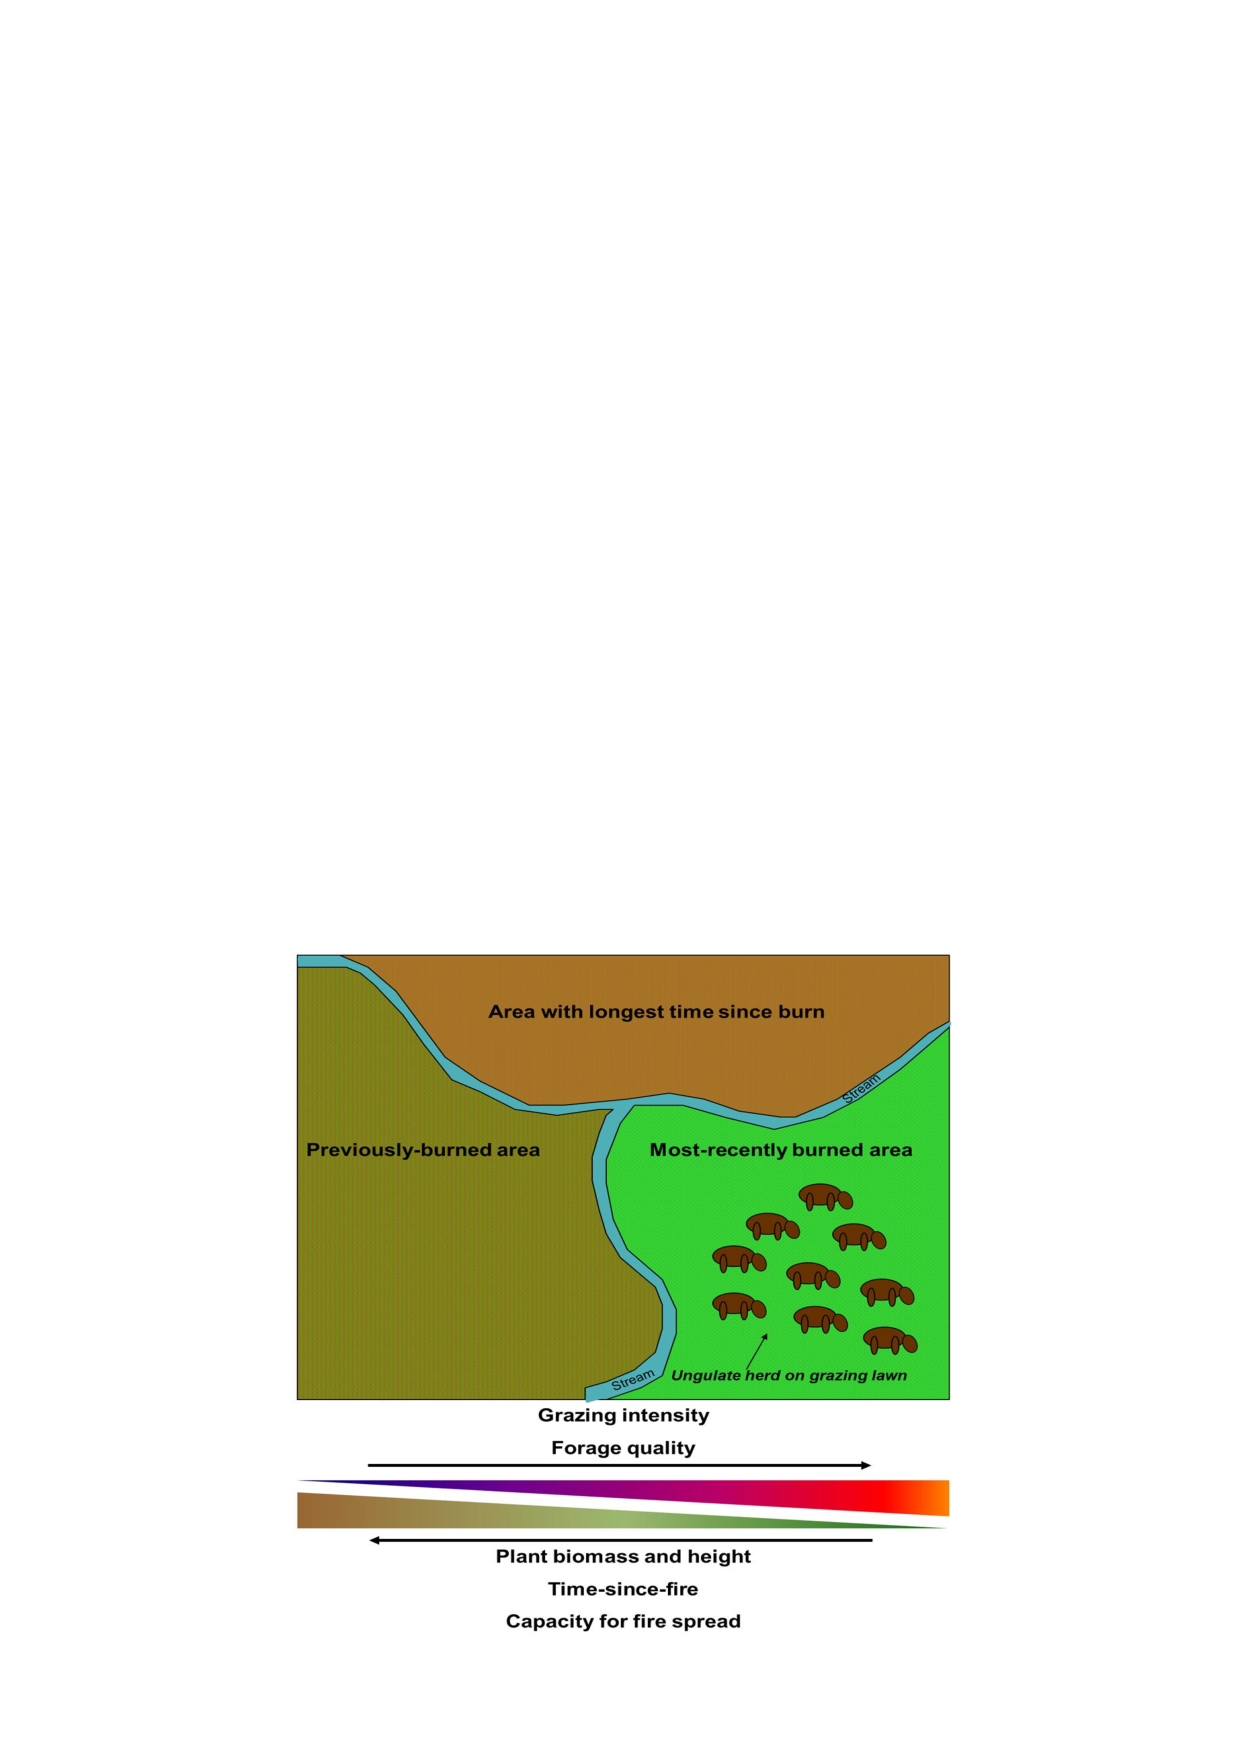
\includegraphics[width=1\columnwidth]{FireGrazingInteraction}
	\caption[The fire-grazing interaction]{A stylized representation of landscape-level patterns associated with coupled fire and grazing regimes originally presented by \citet{mcgranahan2013b}.}
	\label{fig:FGI}
\end{figure}

Grazers seek out recently-burned areas and concentrate their herbivory and physical impacts in those patches, responding to the "magnet effect" created by the high nutritive quality and overall high palatability that characterizes post-fire plant regrowth \citep{archibald2005, allred2011b}. 
Meanwhile, grazers generally avoid unburned areas, allowing these patches to reach later successional stages and accumulate aboveground plant biomass useful for wildlife that prefers dense vegetation until those patches, with their higher fuel loads, carry subsequent fire (Fig.~\ref{fig:FGI}). 
The result is a spatially and temporally variable "shifting mosaic" across the landscape driven by fire and grazing that increases niche diversity for rangeland wildlife \citep{fuhlendorf2004, fuhlendorf2006, hovick2014}. 

When managers of working rangeland landscapes shift objectives from maximizing livestock production to enhancing the delivery of multiple ecosystem services, a frequent strategy is restoring pre-settlement pattern and processes. 
Specifically, rangelands benefit from the restoration of the shifting mosaic of vegetation structure via re-coupling the fire-grazing interaction \citep{fuhlendorf2012}. 
Not only does landscape-level heterogeneity create a broader range of habitat for grassland-obligate species in space (Fig.~\ref{fig:habitat}), but spatial heterogeneity stabilizes ecological structure and function by reducing temporal variability \citep{fuhlendorf2017}. 
Especially in the context of management, the implementation of pyric-herbivory is known as \emph{patch-burn grazing} \citep{fuhlendorf2004, mcgranahan2012}. 

\begin{figure}[!b]
	\center
	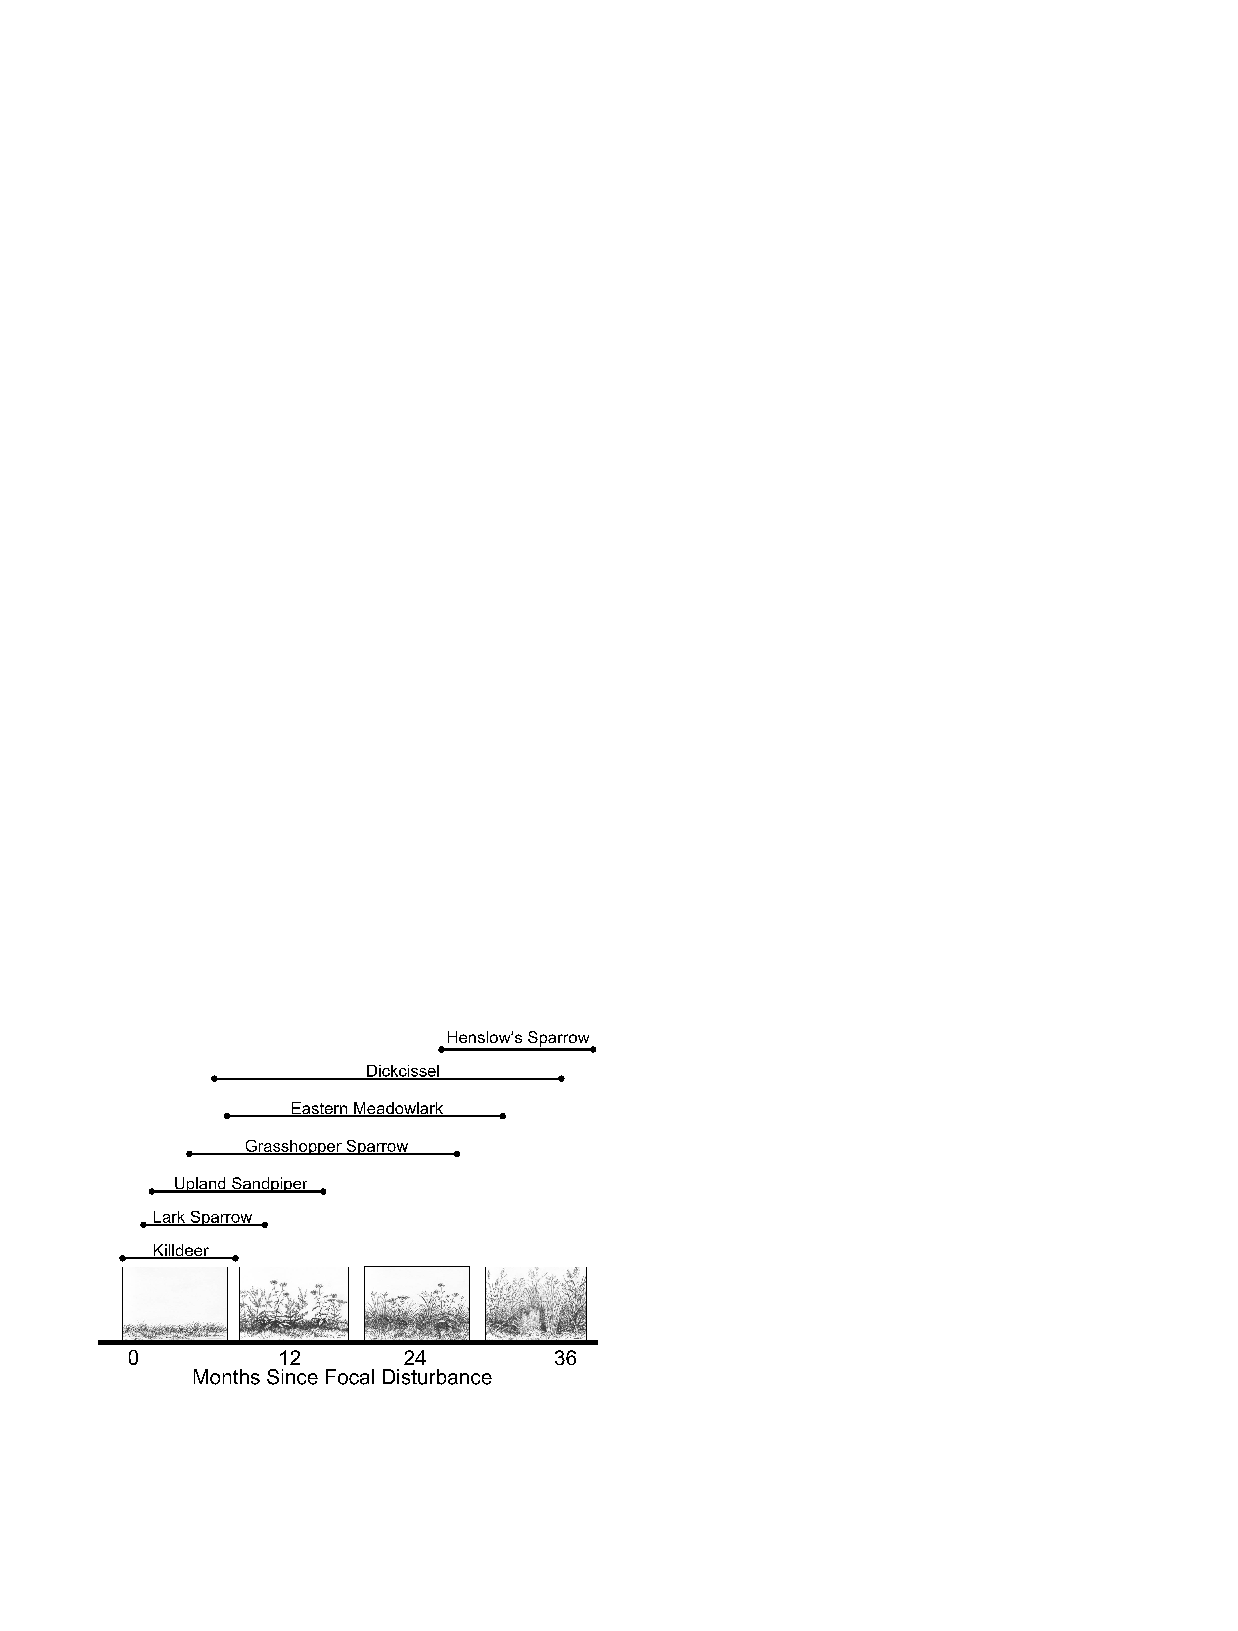
\includegraphics[width=1\columnwidth]{PBGhabitat}
	\caption[Vegetation structure, grassland birds, and the fire-grazing interaction]
	{Vegetation structure varies with time-since-fire and creates a gradient of distinct habitat types that are each required by different species of grassland-dependent wildlife. 
	Recently-burned patches are characterized by short stature as grazers focus on high-quality post-fire regrowth. 
	Grazers ignore patches with longer time-since-fire, which allows those areas to develop rank material used by other species and increase the probability of carrying fire after subsequent ignitions.
	Widely used in the pyric-herbivory literature, this version of the figure came from \citet{fuhlendorf2009}.}
	\label{fig:habitat}
\end{figure}

Large conservation-focused units in the Great Plains have also sought to restore fire-grazing interactions; it is not limited to working landscapes and commercial ranches. 
For example, in the Flint Hills of Kansas (known as the Osage in Oklahoma), both the Nature Conservancy's Tallgrass Prairie Preserve and the NPS Midwest Region's Tallgrass Prairie National Preserve have implemented prescribed fire management programs in their grazed landscapes designed to promote the interaction of fire and herbivory \citep{hamilton2007, leis2013}. 

\paragraph{Implementation \& management}

It is significant for our recommendations that Tallgrass Prairie National Preserve (TAPR) has successfully managed an interactive fire and grazing management regime with patch-burn grazing. 
It demonstrates that not only can ecological disturbance regimes be coupled on NPS land, but management perspectives and personnel can be synchronized, as well. 
However, the TAPR is an ecological outlier in the Midwest Region, given that all other units are located both farther west and farther north in cool-temperate climate zones dominated by northern mixed-grass prairie. 
Furthermore, the historical context of ranching that is brought so heavily to bear in the TAPR's cultural preservation (e.g., barns on-site) and inclusion of livestock grazing also includes a regionally-unique appreciation for the role of fire in rangeland ecosystems. 

Despite a similar evolutionary history of fire in the northern mixed-grass prairie, prescribed fire has a much lower cultural status among residents of the region. 
From politicians to landowners, fire is viewed much more skeptically and is considered a very limited tool, rather than a necessary ecological process. 
This is a fundamental barrier to prescribed fire use on NPS units in the northern mixed-grass prairie and demands further research from the social science side of natural resource management. 

Despite the positive model for pyric-herbivory on NPS land offered by TAPR, we posit coupled fire-grazing regimes on other NPS units in the Midwest Region are better modeled on the TNC's Tallgrass Prairie Preserve (TPP) in northeastern Oklahoma.
In the main bison unit of the TPP, the desired aesthetic reflects more the shifting mosaic of disturbance-driven patches across a broad landscape, rather than the discrete patch contrast created by burning subsets of pastures as in patch-burn grazing as implemented by TAPR. 
Facilitated by a much larger spatial area, the TPP makes use of natural fire breaks to delineate non-angular burn patches and burns throughout the year and under a certain degree of randomness in spatial burn unit selection to effect a "messy" landscape in which the human agency behind the disturbance regime is less obvious.
We suspect this aesthetic is more consistent with the visitor experience sought by NPS units in the Midwest Region outside of the TAPR.

\paragraph{General considerations}

\subparagraph{Fire return interval}

An important step in formulating managed fire regimes is the desired \emph{fire return interval}\textemdash the duration of time between prescribed fires. 
Fire return interval is synonymous with fire frequency, reported as the number of burns within a specific period of time. 
The main ecological consequence of fire frequency relates to succession. 
Longer fire return intervals allow greater time for successional dynamics to play out in the plant community. 
Generally speaking, in grasslands, the potential bounds of fire frequency are determined by fuels.
Fires cannot occur more frequently than fuel accumulation allows an ignition to spread. 
Thus, more arid areas typically have longer fire return intervals than wetter areas. 
For areas with sufficient rainfall and without other disturbance, lengthy fire return intervals allow woody plants to establish.
Should woody plants reach such a density that herbaceous species decline, fire regime shifts with the plant community, likely away from frequent surface fires to infrequent surface fires and/or high-severity canopy fires. 

Appropriate fire return intervals can be determined via two main approaches. 
The typical approach, especially for conservation areas, is to determine the "natural" fire frequency for the area under the desired conditions to be conserved or restored to. 
In general, the North American Great Plains are believed to have burned, on average, once every 3-10 years, with longer fire return intervals in drier, less productive, and cool-temperate (northern) sub-regions. 

Another approach to determining appropriate fire frequency is to emphasize the management needs of the area in question. 
This is especially relevant for the initial phases of rangeland restoration or the continued management of \emph{novel ecosystems}\textemdash ecosystems in which the plant composition or other ecological dynamics lack a known ecological analog. 
A regional example of novel ecosystems might be rangelands heavily invaded by Kentucky bluegrass (\emph{Poa pratensis}) or other cool-season invasive grasses, which introduce novel fuel components (excessive thatch or high-moisture live biomass; \citet{toledo2014a, mcgranahan2012a}). 

Obviously, the two approaches can be combined. 
For example, estimations of "natural" fire frequency often span wide ranges, and specific fire return intervals within those bounds can be informed by management objectives. 

Successfully coupling fire and grazing disturbance regimes requires target fire return intervals to be established as a means to determine how much of an area should be burned each year. 
A basic tenet, of course, is that fire must occur each year to provide high-quality forage for grazers and subsequent low-stature vegetation for wildlife.
In a simplified patch-burn grazing system, a manager simply burns one-third of a pasture to achieve a three-year fire return interval, or one-quarter of the pasture to achieve a four-year fire return interval. 

The situation is less clear on large, open conservation areas supporting herds of native grazers in a natural setting, which is why we suggest TNC's Tallgrass Prairie Preserve is likely a better model for the NPS Midwest Region than even the Region's own Tallgrass Prairie National Preserve. 
The TPP manages a much more "messy" system in which fire return intervals are actual averages over time and space, with some burn units burning slightly more or less frequently than prescribed. 

\subparagraph{Stocking rate and forage utilization} Once the size of annual burn \emph{area} is determined from the target fire \emph{frequency} within the \emph{extent} of the grazing unit, one must determine the desired number of grazers. 
Any sustainable stocking decision-making ensures that the grazing demand does not exceed the forage available. 
In general, successfully coupling fire and grazing regimes involves additional considerations, and doing so within the context of grazing ecosystem conservation and native herbivore management on NPS properties, specifically, raises further challenges. 
Many of these are discussed below. 
But independent of management objectives and resources, decision-making for sustainable stocking is impossible without robust data on forage availability. 
Thus, we discuss below existing data gaps and how they can be addressed within the framework of coupled fire and grazing regimes. 
The process begins with basing burn unit delineations on expected plant community responses. 

\subsection{Burn units based on ecological sites}

Effective management of grazing ecosystems based on a strategy of coupled fire and grazing regimes requires information about vegetation that our research indicates is absent from NPS decision-making in the Midwest Region. 
Furthermore, based on our data audits of NPS units in the region, it does not appear that relevant data are available even if they were to be included in decision-making processes. 

Here, we describe data necessary to inform robust delineation of prescribed fire units that support forage resources and a sustainable and resilient grazing ecosystem. 
We also outline protocols to both establish baseline information on forage production and monitor responses to the restoration of coupled fire and grazing. 

\subsubsection{Establishing site productivity}

Rangelands in the western United States are delineated by \emph{ecological sites}, which the USDA NRCS   \href{https://www.nrcs.usda.gov/wps/portal/nrcs/detail/national/landuse/rangepasture/?cid=stelprdb1068392}{defines as}

\begin{quote}
	... a distinctive kind of land with specific soil and physical characteristics that differ from other kinds of land in its ability to produce a distinctive kind and \emph{amount of vegetation} and its ability to respond similarly to management actions and natural disturbances. 
\end{quote}

We've added the emphasis on \emph{amount of vegetation} to highlight the central role that ecological site descriptions\textemdash ESDs, or the ecological information assembled for each ecological site\textemdash play in sustainable rangeland management. 
ESDs include information about annual aboveground primary production by plant species and functional group, at monthly intervals through the growing season. 
When weighted by the area within a unit each ecological site represents, these productivity data give valuable insight into total forage production and thus the number of grazing animals the unit can support. 

We recommend NPS units in the Midwest Region incorporate ecological site descriptions into decision-making processes to support a strategy of sustainable grazing ecosystem management. 
Our research indicates that ecological sites are not currently in use at all within the study region. 
The system is either unknown to managers, or considered too fine-scale to inform management of areas as large and environmentally variable as national parks. 
This is a legitimate concern that has been already been addressed in rangeland science. 
\citet{stringham2016} increased the utility of fine-scale ecological site descriptions by identifying \emph{disturbance response groups} that combine similar ecological sites into broader landscape delineations. 
A similar approach could be applied to each Midwest Region NPS unit.

The primary means by which ecological site information should be applied is in the delineation of burn units. 
Coupling fire and grazing regimes requires that grazers find sufficient forage in burned areas to support their energetic requirements. 
Other considerations for stocking are discussed below. 
When relying on burned patches for sufficient forage quality and availability, it is essential that the plant communities be sufficiently diverse to provide stable productivity from season to season and from year to year. 
This is best achieved by taking advantage of the selection effect, delineating burn units that are equally represented by highly-productive ecological sites.
 
A poor example of burn patch delineation would be a burned area in one year that encompasses most of the spatial distribution of highly-productive, bottomland sites, and in another year a burned area that is almost entirely thin upland sites. 
Such differences in productivity are especially sensitive to climate variability. 
For example, if the year in which the lowland sites are burned is particularly high in precipitation, forage production is at risk of exceeding the ability of grazers to maintain short stature in the burned patch, resulting in a loss of the fire-grazing interaction (condition A, fig.~\ref{fig:stocking}). 
Likewise, if the year in which the burned patch comprises mostly upland sites has particularly low precipitation, forage production will fall substantially below grazer requirements and sites will be overgrazed (condition C, fig.~\ref{fig:stocking}). 
Thus, interannual variability is mitigated by ensuring burn units include a diversity of ecological sites. 

\begin{figure*}[t]
	\begin{minipage}{0.55\textwidth}
		\raggedright
			\caption[Optimal stocking to couple fire and grazing]
		{Successfully coupling fire and grazing regimes requires a moderate stocking rate (B) that matches grazer offtake to vegetation production. 
			Under excessive stocking (C), the fire-grazing interaction is weakened as grazers are forced to forage beyond the perimeter of the burned patch. 
			The consequences of overstocking are intuitive: poor grazer performance and excessive severity to the plant community. 
			Less intuitive\textemdash especially in the context of conservation grazing\textemdash are the consequences of understocking (A). 
			If plant production exceeds the capacity of grazers to consume the available forage, vegetation will reach maturity and subsequent declines in forage quality risks weakening the magnet effect that concentrates grazers to burned patches. }
		\label{fig:stocking}
	\end{minipage}
~~
	\begin{minipage}{0.4\textwidth}
		\flushright
	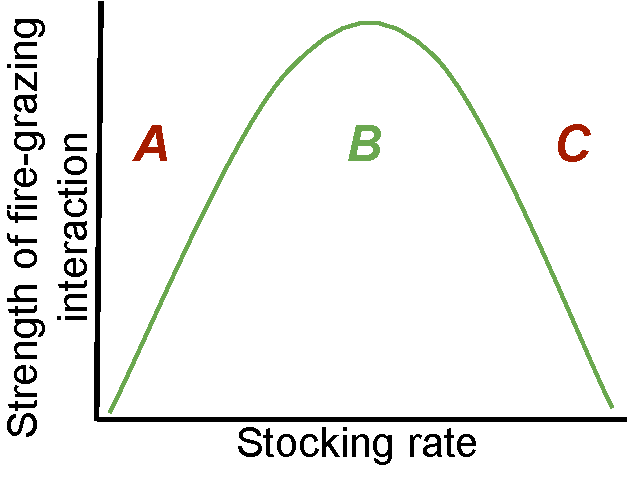
\includegraphics[width=1\textwidth]{stocking}
	\end{minipage}
\end{figure*}

\subsubsection{Necessary vegetation data}

Making these decisions requires site-specific knowledge of plant community composition and productivity. 
Given the unique conservation objectives and management of NPS units compared to working rangeland (e.g., privately-owned rangeland, US Forest Service or other federal grazing allotments), we suggest it should not be assumed that vegetation dynamics on NPS units are optimally reflected in existing ecological site descriptions. 
Thus we recommend Midwest Region NPS units initiate a concerted ground truthing effort to verify plant community phases and productivity on at the level of individual ecological sites.
These data could then easily support a subsequent effort to identify disturbance response groupings \citep[as per][]{stringham2016} that would ultimately be used as the basic unit of landscape management.
Once vegetation status is established, less-intensive sampling within disturbance response groupings can be conducted over time to monitor potential community phase transitions in response to management. 

Two models exist for initial data collection within ecological sites and subsequent monitoring of disturbance response groupings. 
Firstly, Dr. Kevin Sedivec in North Dakota State University's Range Science Program developed a protocol for the Little Missouri National Grasslands to verify soil series, vegetation composition, and annual primary productivity within grazing allotments. 
This is an intensive protocol in which (1) a soil pit is dug to verify the soil series on which the ecological site identification is based, and (2) aboveground vegetation is clipped by species to determine species-level productivity. 
Such an intensive protocol would only be required to establish the current state of plant communities on ecological sites in Midwest Region NPS units, and could be scaled back substantially. 

Secondly, \citet{symstad2012} developed a protocol for plant community composition and structure monitoring with the aim to

\begin{quote}
	provide park managers with early warning of undesirable change, measure digression from or progress towards a desired state, and evaluate effectiveness of management programs.
\end{quote}

The protocol was recently used in the Midwest Region, at Badlands National Park \citep{ashton2019}. 
Although the protocol does not specifically sample for aboveground plant biomass production, clipping data from representative plant communities could easily calibrate the species composition data obtained via point-intercept methods \citep{yurkonis2012}.
We strongly encourage managers in the NPS Midwest Region to consider how this protocol could be adapted to initially ground-truth ecological sites and subsequently monitor disturbance response groups to support fire and grazing management. 

\subsection{Stocking for sustainability}

Sustainable grazing management\textemdash critical to the health of grazing ecosystems in NPS units\textemdash essentially relies on matching grazer demand to forage availability. 
Above, we discuss above how information on plant productivity can inform the delineation of burn units to stabilize the forage availability side of the stocking equation. 
Here we discuss two aspects of grazing management that will likely arise in the pursuit of coupled fire and grazing regimes and potentially contrast with established modes of thinking about conservation grazing: the importance of domestic livestock, and apparent grazing severity. 

\subsubsection{Domestic livestock}

The Midwest Region NPS must not overlook the conservation value of domestic livestock in sustainable grazing ecosystem management.
Unfortunately there is persistent conventional wisdom regarding livestock grazing on public lands that primarily associates domestic grazers with degradation \citep{fleischner1994}. 
But it is important to remember that \emph{grazing management} has greater influence on environmental impacts than \emph{grazer identity}, and that well-managed cattle grazing has been shown to advance rangeland biodiversity management goals in the Great Plains \citep{ahlering2016, allred2011}. 

As such, cattle grazing facilitated by co\"{o}peration with local ranchers should be viewed as a potent and flexible resource for the sustainable management of grazing ecosystems in Midwest Region NPS units. 
In its most obvious application, co\"{o}perative grazing agreements can ensure grazing disturbance on NPS units that do not currently have bison filling the large herbivore niche. 
Less obviously, co\"{o}perative grazing agreements potentially serve as a flexible resource for managers to adjust grazing intensity from year to year or even within grazing seasons, depending on precipitation and grassland resource response to "baseline" grazing pressure from resident bison herds. 

While there are several approaches to managing stocking rates, given the importance of maintaining a minimum level of grazing intensity in burned areas, we recommend Midwest Region NPS units adopt an opportunistic stocking strategy. 
We specifically recommend the "tracking" strategies described by \citet{campbell2006} in which stocking rates are varied in response to precipitation to protect against overgrazing in dry years and under-utilization in wet years. 
\citet{campbell2006} outline two tracking strategies: 

\begin{itemize}
	\item \emph{Low-tracking}\textemdash a conservative strategy in which stocking rates are always kept below the ecological carrying capacity and vary based on rainfall.
	\item \emph{High-tracking}\textemdash in which managers attempt to maintain stocking rates at the ecological carrying capacity and vary based on rainfall.
\end{itemize}

The high-tracking strategy might be preferable given grassland resources across Midwest Region NPS units are generally under-utilized, and management would benefit from a stronger influence of grazing disturbance. 
Whether NPS units have the capacity to make the necessary adjustments to match stocking rate to forage availability likely depends on their willingness to include domestic livestock in grazing ecosystem management. 
NPS units are unique among grazing land managers in that the objective is to maintain populations of native herbivores in natural settings. 
This reduces flexibility and responsiveness in stocking rate management, as it is logistically challenging to increase or decrease herd sizes, especially within grazing seasons. 

We suggest a hybrid approach to bison grazing management that includes regional satellite herds and domestic livestock. 
\emph{In NPS units with core bison herds,} bison should be considered the primary grazers and annual stocking rates set just below ecological carrying capacity. 
If reductions are necessary, animals can be transferred to satellite herds. 
Additional grazing up to the ecological carrying capacity can be facilitated by spatially- and temporally-targeted livestock grazing. 
Meanwhile, \emph{NPS units without core bison herds} would consider livestock their primary grazers and adjust livestock numbers to accommodate whatever bison they take on as a satellite herd, if any. 
We realize such an approach likely constitutes a radical departure from current management perspectives, resource allocations, considerations for visitor experience, and perhaps even policy. 
Nonetheless we suggest it as a means to generate novel thinking and ideally novel approaches to active grazing management. 
 

\subsubsection{Grazing severity} 

Another counter-intuitive component of sustainable grazing ecosystem management is that successful restoration of the fire-grazing interaction will likely bear signs of grazing that many in the conservation community have been conditioned to interpret as indicators of degradation rather than optimal ecological function. 
In this sense, the key take-home of the relationship between stocking rate and the successful coupling fire and grazing (Fig.~\ref{fig:stocking}) is not the optimality of moderate stocking, but the requirement that a minimum level of grazing intensity be maintained.
Thus, it is entirely possible to stock too lightly such that grazers lose body condition and vegetation degrades.

Ensuring that grazing activity matches plant production begins with setting stocking rates with respect to the expected productivity of the \emph{entire grazing unit}, even though it is anticipated that grazers focus the majority of their activity within \emph{burned patches}. 
A misconception among managers of conservation areas regarding patch-burn grazing is that stocking rates be set based on the burned patch alone, but the result will likely be understocking and a weak fire-grazing interaction as in condition A in Figure~\ref{fig:stocking}. 
Furthermore, grazers will fail to maintain the low vegetation structure sought for grassland biodiversity (Fig.~\ref{fig:habitat}).

Proper stocking in a coupled fire-grazing system creates high-impact grazing in the burned patch, which is necessary to maintain desired vegetation structure.
The key is that native prairie plant communities have evolved to tolerate high-intensity grazing for a season or two. 
As long as the shifting mosaic creates another burned area to draw grazers away in subsequent seasons, such high-intensity grazing will not have lasting effects on plant community composition or productivity. 

Managers and visitors alike might balk at what appears to be severe over-utilization in discrete areas. 
Substantial buy-in and understanding among NPS staff and targeted interpretative educational materials will likely be required to ensure the appearance of success in restoring a functional grazing ecosystem is not misinterpreted. 